\chapter{SMACK Verification Framework}\label{ch:smackframework}
SMACK is part of a modular software verification framework which is
built on top of the Boogie intermediate verification language (IVL),
and aims to reduce the large engineering effort typically required for
implementing bounded software verification tools.  This chapter first
provides some background for SMACK's verification framework, then
introduces the SMACK toolchain, and finally, discusses the
environment presented by the framework for modeling input program
behavior.  

\section{Framework Background}
Developing a fully featured bounded software verification tool from
end-to-end can be a daunting task.  Bounded model checking requires
several steps.  First, the input source code must be parsed or
compiled.  The resulting abstract syntax tree (AST) must then be
semantically interpreted, and a model built of underlying program
semantics. Finally, the modeled program must be represented as a
satisfiability modulo theories (SMT) query and passed through an SMT
solver.  This imposes a large barrier to entry for prototyping a new
model checking algorithm, or building a verification tool for a new
source language using existing algorithms. 

The Boogie intermediate verification language (IVL) was designed by
Microsoft Research to alleviate the complexity of modeling new source
languages and implementing new model checking algorithms.  Boogie IVL
separates the task of modeling input program semantics from the task
of bounding and checking modeled programs.  This allows model checking
tools to take Boogie IVL files as input, rather than the input source
language.  Similarly, front-end tools can model the input program
semantics in Boogie IVL rather than being directly integrated with
the model checker.  By providing a layer of abstraction between the
tasks of modeling input source programs and the checking of modeled
programs, Boogie IVL enables the development of components in a
modular fashion.  The resulting components can be roughly separated
into two categories: front-end modeling tools, and
back-end solvers.

\subsection{Front End Modelers}\label{sec:frontends}
Due to its goal of creating an abstraction between program modeling
and model checking, Boogie IVL has been designed to be a very
low-level modeling language.  It contains support for little more than
a typing system, basic arithmetic expressions \& statements, control
flow \& procedure calls, and verification condition
specification~\cite{boogie}.  Any more complicated semantics of the
source language must be modeled using the basic set of primitives
available in Boogie IVL.

Though the low-level nature of Boogie IVL provides the flexibility to
support a large variety of models of computation and source languages,
it requires that models be created to define the semantics of
operations available within the source language and computational
model environments.  As an example, there is no concept of a heap
within Boogie.  Because of this, a memory model must be developed that
accurately models the behavior of the heap.  A rudimentary model of
memory could use a simple, large array of integers to represent the
heap, where each element represents a word of memory, and C pointers
are simply indices into this array.

The SMACK tool itself, which translates C/C++ code into Boogie IVL, is
one example of a front-end for this framework.  There are several
other front-ends, which provide support for mainstream programming
languages such as .NET and Java, in addition to verification and
prover languages like Dafny and Chalice.

\subsection {Back End Solvers}
The original back-end solver for Boogie IVL programs is a tool called
Boogie.  (To ease discussion, ``Boogie'' will hereafter refer to
Boogie IVL, while ``Boogie verifier'' will refer to the back end
solver.)  In addition to being a complete back-end verifier for Boogie
programs, it also provides an API for parsing Boogie IVL and 
interfacing with SMT solvers. As the goal of Boogie is to modularize
model checking verifiers, it should not be surprising that there are
several additional back-end solvers that perform verification of
Boogie programs, such as Corral and Duality.  

Corral is one of the more popular back-end solvers for Boogie
programs, and also happens to be an excellent example of how Boogie
has simplified the implementation of new model checking algorithms.
Corral leverages the Boogie verifier's API to parse Boogie code and
interface with SMT solvers~\cite{corral}.  However, Corral implements
model checking algorithms not available with the Boogie verifier, such
as the Lal/Reps sequentialization algorithm~\cite{LalReps}. Indeed,
Corral has put considerable effort toward providing support for
verification of concurrent programs.  As such, it was the ideal
candidate to use as a back-end verifier for the pthreads extension of
SMACK. 

However, although providing state of the art algorithms for checking
concurrent programs, Corral is similar to the Boogie IVL in that it
provides only low-level support for modeling concurrency.  The Corral
program verifier provides an extension to Boogie IVL that includes a
very basic set of primitives for modeling concurrent programs.  The
behavior prescribed in the pthread specification~\cite{pthreads} is
much more complex than these low-level concurrency primitives
recognized by Corral.  As a result, to provide support for the more
complex pthread API within SMACK, it is necessary to build a model
capturing the behavior of the pthread API, using the primitives
provided by Corral. 


\section{SMACK Toolchain}\label{sec:smacktoolchain}
As mentioned in Section~\ref{sec:frontends}, the SMACK tool itself is
a front-end for the verification framework centered around Boogie.
However, at its core, it is essentially a compiler that takes C/C++
programs and translates them into Boogie IVL~\cite{smack}.  This
converted Boogie code is then consumed by a back-end solver, which
evaluates verification conditions present in the original source
code.

To stitch all of this together, the SMACK project defines a toolchain
that drives the entire process.  In conjunction with one of several
supported back-end solvers, this makes SMACK an end-to-end bounded
software verification tool for C/C++ programs.

\begin{figure}[!ht]
  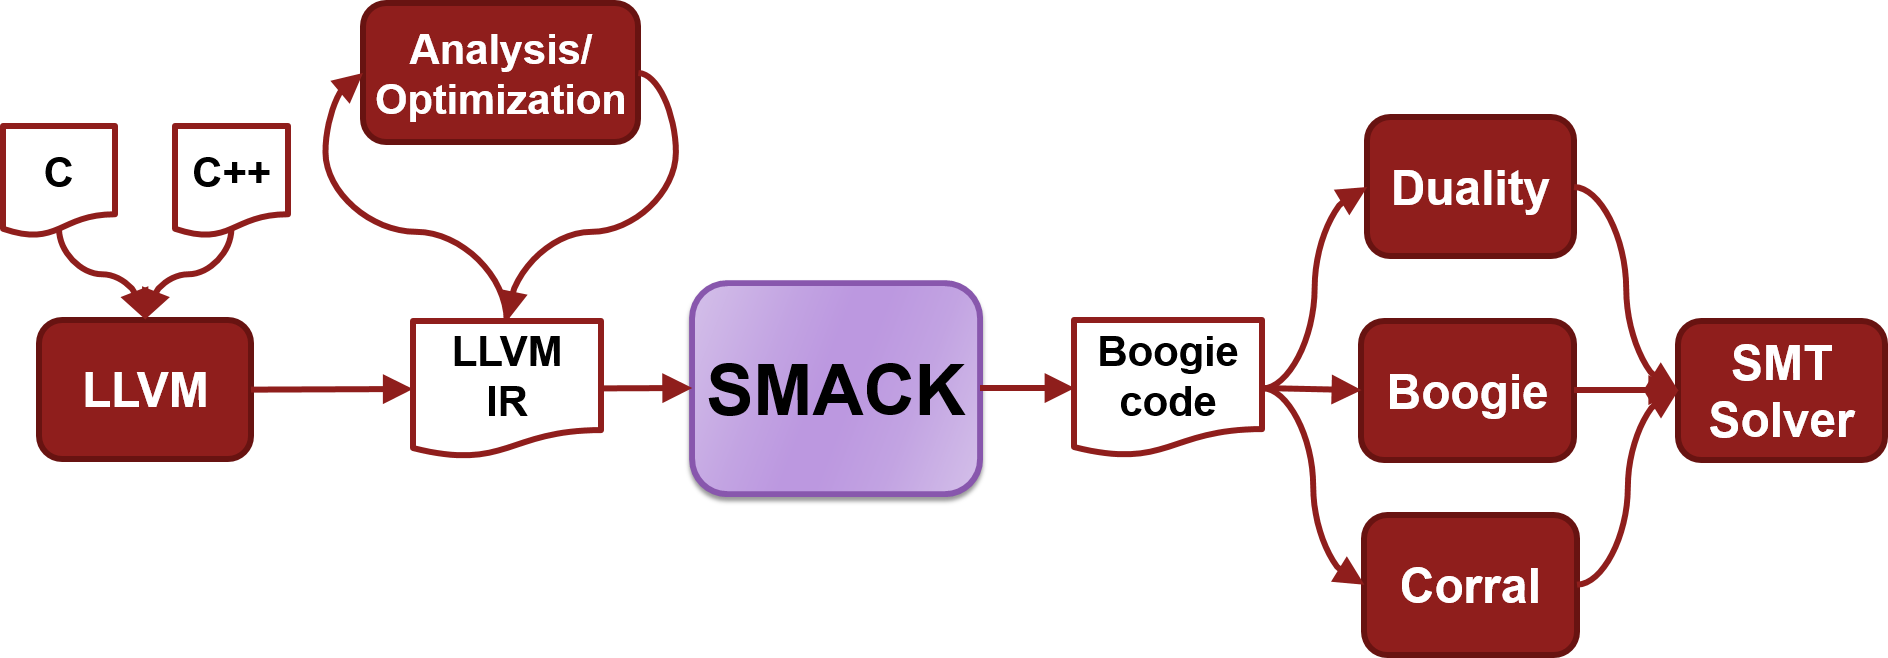
\includegraphics[width=1\textwidth]{SmackToolchain.png} 
  \caption{SMACK Toolchain}
  \label{fig:SMACKToolchain}
\end{figure}

The SMACK toolchain is depicted in Figure~\ref{fig:SMACKToolchain}.
Input C/C++ programs are given to Clang to compile and link, resulting
in an LLVM bytecode output.  This is then passed to the SMACK
executable, which translates the LLVM bytecode into a Boogie program
that models the behavior of the input C/C++ program.  The resulting
Boogie program is then passed to the back-end solver.  The solver
converts the Boogie program into an SMT query, which is then given to
one of the SMT solvers supported by the back-end solver for
evaluation. 

\section{Modeling Environment}\label{sec:modelingenvironment}
As described in Section~\ref{sec:smacktoolchain}, SMACK consumes LLVM
IR bytecode, builds a model of the input program, and generates a
Boogie IVL model of the input program.  The design of this toolchain
provides several levels at which modeling semantics can be
introduced. At the C level, external library functions that are
otherwise undefined can be given a definition, rather than verifying
the entire original source library. At the SMACK translation level,
undefined functions can be intercepted so SMACK can perform predefined
alterations to the translated Boogie program, rather than being
directly translated from the LLVM IR representation.  At the
translated Boogie level, additional variables and instructions can be
added to model environmental functionality that is not defined at the
C level. Finally, additional functionality can be modeled by the
back-end solver itself. 

To provide some context for the discussion of the modeling process,
the remainder of this chapter briefly introduces Boogie IVL, and then
discusses the mechanisms used for modeling, such as the Corral
concurrency primitives and C level Boogie injection.

\subsection{Boogie IVL}
The most illustrative way to introduce Boogie IVL is to simply show an
input C program and the relevant portions of the Boogie output that
SMACK returns. 
\begin{figure}[!ht]
\centering
\begin{subfigure}[b]{.45\textwidth}
\centering
\begin{lstlisting}


void main() {
  int *x, *y;
  x = malloc(sizeof(int));
  y = malloc(sizeof(int));
  *x = 1;
  *y = 2;
  assert(*x == 1);
}
\end{lstlisting}
\caption{Input C Code}\label{fig:cToBoogie_a}
\end{subfigure}
~
\begin{subfigure}[b]{.45\textwidth}
\centering
\begin{lstlisting}[language=boogie]
var $M: [int]int;

procedure main() {
  var $x, $y: int;
  call $x := $malloc(4);
  call $y := $malloc(4);
  $M[$x] := 1;
  $M[$y] := 2;
  assert($M[$x] == 1);
}
\end{lstlisting}
\caption{Boogie Code from SMACK}\label{fig:cToBoogie_b}
\end{subfigure}
\caption{SMACK Translation of C Program}\label{fig:cToBoogie}
\end{figure}

Figure~\ref{fig:cToBoogie_b} shows a reduced version of the Boogie
code as translated by SMACK from the input source depicted in
Figure~\ref{fig:cToBoogie_a}.  This simple program allocates space for
\lstinline|x| and \lstinline|y| on the heap, assigns values to each,
and then \lstinline|assert|s that the value of \lstinline|x| is as it
was assigned.  The Boogie translation reflects this, allocating space
on a model of the heap, \lstinline|$M|, and then indexing into this
array when storing and loading dynamic memory values.

\subsection{Corral Concurrency Primitives}
Corral is a state of the art solver for Boogie IVL programs.  One of
Corral's recent development efforts has been to improve support for
verifying concurrent programs.  To this end, Corral has extended
Boogie IVL, and recognizes the following concurrency primitives:

\begin{itemize}
\item \lstinline|async call|
  \emph{func}\lstinline|(|\emph{...}\lstinline|)| -- Asynchronously
  calls \emph{func} with the parameter list \emph{'...'} 
\item \lstinline|corral_atomic_begin()| -- Begins an atomic block
\item \lstinline|corral_atomic_end()| -- Ends an atomic block
\item \lstinline|corral_getThreadID()| -- Returns the ID of the
  calling thread.
\item \lstinline|corral_getChildThreadID()| -- Returns the ID of the
  most recently spawned thread
\end{itemize}

\begin{figure}[!ht]
\centering
\begin{lstlisting}[language=boogie]
var $x: int;
procedure f() modifies $x; {
  var $tid, $tmp: int;
  call $tid := corral_getThreadID();
  call corral_atomic_begin();
  $x := $tid;
  $tmp := $x
  call corral_atomic_end();
  assert($tmp == $tid);
}
procedure main() {
  var $ch1, $ch2: int;
  $x := 0;
  async call f();
  $ch1 := corral_getChildThreadID();
  async call f();
  $ch2 := corral_getChildThreadID();
  assert($x == $ch1 || $x == $ch2);
}
\end{lstlisting}
\caption{Utilizing Corral Concurrency Primitives}
\label{fig:corralprimitives}
\end{figure}


Figure~\ref{fig:corralprimitives} demonstrates the usage of each of
these primitives within the context of a complete Boogie program.
This program initializes the global variable \lstinline|$x| as 0, then
makes two asynchronous calls to the function \lstinline|f()| and
records the thread ID of each of the spawned threads of execution.  In
\lstinline|f()|, each of the spawned threads records their thread IDs.
Each thread then starts an atomic block, where it stores its thread ID
to the global \lstinline|$x| and then loads global \lstinline|$x| into
the local variable \lstinline|$tmp|.  The \lstinline|assert()| in
\lstinline|f()| should always succeed, since \lstinline|$x| is stored
and loaded within an atomic block. 

However, this program contains a bug.  Because there is no barrier
forcing the parent to wait for the child threads to execute, it is
possible that \lstinline|$x| will not be set to the thread ID of
either children by the time \lstinline|assert()| is called in
\lstinline|main()|.

\subsection{C Level Modeling}\label{sec:clevelmodeling}
Because there are several layers at which model semantics can be
introduced, SMACK has introduced several special C level functions
which insert model semantics at these various layers.
These special C level functions are not directly translated into
Boogie code, but, instead, are processed specially by SMACK.  This
allows users to introduce program semantics at the lower levels of the
modeling environment by writing code at the C level.  As a result, OS
environment and library models can be completely written as libraries
which get included C by input programs.  This avoids modifying SMACK's
source code directly in order to implement such models.

There are several C level functions that SMACK treats specially when
seen in the LLVM IR AST.  Upon seeing these, SMACK performs special
transformations to the Boogie translation, rather than translating the
function calls as they are.  Two of these functions were particularly
important for modeling the pthread extension to SMACK.

\begin{itemize}
\item \lstinline|__SMACK_code(char* format, ...)| -- Injects the
  string \lstinline|format| in the Boogie code.
\item \lstinline|__SMACK_top_decl(char* format, ...)| -- Inserts the
  string \lstinline|format| as a global declaration 
\end{itemize}

\begin{figure}[!ht]
\centering
\begin{subfigure}[b]{1\textwidth}
\centering
\begin{lstlisting}
void main() {
  __SMACK_top_decl("var $globalVar: int;");
  int *x;
  x = malloc(sizeof(int));
  *x = 1;
  __SMACK_code("$globalVar := @", *x);
  __SMACK_code("@ := $globalVar + 1", *x);
  assert(*x == 2);
}
\end{lstlisting}
\caption{Boogie Injecting C Code}\label{fig:cinjToBoogie_a}
\end{subfigure}
~
\begin{subfigure}[b]{1\textwidth}
\centering
\begin{lstlisting}[language=boogie]
var $globalVar: int;
var $M: [int]int;

procedure main() {
  var $x: int;
  call $x := $malloc(4);
  $M[$x] := 1;
  $globalVar := $M[$x];
  $M[$x] := $globalVar + 1;
  assert($M[$x] == 2);
}
\end{lstlisting}
\caption{Injected Boogie Translation}\label{fig:cinjToBoogie_b}
\end{subfigure}
\caption{Injecting Boogie Code from C}\label{fig:cinjToBoogie}
\end{figure}

Input to both of these functions is similar to that of C's
\lstinline|printf()| function; ``@'' symbols in the
\lstinline|format| string are replaced by arguments from the list
``...''.  Figure~\ref{fig:cinjToBoogie} demonstrates the C level usage,
and Boogie level translations of both of these functions.

The new implementation of pthread support for SMACK performs modeling
exclusively at the C code level, using these Boogie injection 
functions to model environmental state where necessary.

%%% Local Variables: 
%%% mode: LaTeX
%%% TeX-master: "thesis"
%%% End: 
